\section{Odbiornik}

Centralną częścią prezentowanego prototypu stanowi odbiornik.
Jego zadaniem jest wysyłanie sygnałów sterujących do nadajnika, zbieranie ultradźwięków z otoczenia oraz przesyłanie 
ich do komputera w celu dalszej analizy.
Odbiornik składa się z części (rysunek \ref{fig:odbiornik_szkic}):

\begin{itemize}
 \item trzech modułów ultradźwiękowych przetwarzających dźwięk na sygnał elektryczny,
 \item płytki prototypowej \textit{stm32f4-discovery} \cite{bib:stm32f4Discovery} odpowiadającej za komunikację z komputerem,
 \item przystawki do \textit{stm32f4-discovery} przystosowującej sygnały elektryczne z modułów ultradźwiękowych
  do poziomów akceptowalnych przez tę płytkę,
 \item ramy, na której umieszczone są moduły ultradźwiękowe.
\end{itemize}


\rysunek{odbiornik_szkic}{Szkic odbiornika}{\label{fig:odbiornik_szkic}}


\section{Budowa i zasada działania odbiornika}

Głównym elementem odbiornika jest płytka prototypowa \textit{stm32f4-discovery} \cite{bib:stm32f4Discovery}.
 Umożliwia ona komunikację wszystkich komponentów z komputerem.
Oparta jest na procesorze STM32F407VGT6 \cite{bib:stm32f407} typu ARM Cortex M4, 
który zawiera trzy 12-bitowe przetworniki
analogowo-cyfrowe umożliwiające próbkowanie z prędkością do \SI{2,4}{MSPS}. Przetworniki te wykorzystane zostały do próbkowania
sygnałów pochodzących z modułów ultradźwiękowych. Procesor umożliwia również komunikację z komputerem przez 
port USB z prędkością \SI{12}{MB/s}. Na płytce prototypowej znajduje również programator
umożliwiający programowanie procesora i jego testowanie za pośrednictwem dodatkowego portu USB.

Na potrzeby odbiornika powstało dedykowane oprogramowanie w C sterujące procesorem.
Zostało ono oparte na bibliotece \textit{stm32 usb 101} \cite{bib:stm32_usb_101}
zapewniającej komunikację z komputerem, do której dodano obsługę przetworników \textit{ADC}.
Program przez port USB dostaje instrukcję, który z czterech głośników ma nadawać, i przekazuje ją
dalej do nadajnika wraz z sygnałem wyzwalającym. Następnie uruchamiane są równocześnie trzy przetworniki \textit{ADC}, które 
próbkują odbierany dźwięk i poprzez DMA zapisują trzy kanały w pamięci procesora.
Częstotliwość pracy przetworników ustawiono na \SI{1,6}{MSPS}, co daje średnio 40 próbek na jeden okres \SI{40}{kHz} sygnału.
Program zapamiętuje \SI{16}{kS} na każdy kanał, co przy prędkości dźwięku \SI{340}{m/s} pozwala zmierzyć odległość
wynoszącą maksymalnie 2,5 metra.

Po zebraniu w sumie \SI{48}{kS}, całość przesyłana jest do komputera w celu dalszej analizy.
Proces powtarzany jest dla każdego z czterech głośników nadajnika, 
co w sumie daje 12 sygnałów, na podstawie których wyznaczona zostaje 
pozycja w przestrzeni oraz orientacja nadajnika.

Cała elektronika osadzona została na ramie w kształcie trójkąta zbudowanej z rur PCV  (rysunek \ref{fig:trojkat}). 
Odległości pomiędzy modułami ultradźwiękowymi są z góry ustalone, co ułatwia dalsze obliczenia.

\rysunek{trojkat}{Szkic ramy odbiornika}{\label{fig:trojkat}}



\clearpage
\section{Budowa modułu ultradźwiękowego}

Odbiornik wyposażony został w trzy moduły ultradźwiękowe, których zadaniem jest 
zbieranie ultradźwięków z trzech różnych  punktów.
Każdy z modułów zawiera przetwornik piezoelektryczny (mikrofon) 40SR-12 \cite{bib:40ST12},
który przetwarza sygnał akustyczny na odpowiadający mu sygnał elektryczny, oraz wzmacniacze operacyjne 
wstępnie zwiększające siłę sygnału, który przesyłany jest dalej do przystawki.
Rysunek \ref{fig:odbiornik_ultra} przedstawia schemat modułu ultradźwiękowego.

\rysunek{receiver}{Schemat modułu ultradźwiękowego.}{\label{fig:odbiornik_ultra}}

Zasada działania: wzmacniacz operacyjny IC1A wraz z kondensatorem C2 i rezystorem R1 pracuje 
jako przedwzmacniacz ładunkowy \cite{bib:wzm_ladunkowy}.
Ładunek wytworzony na przetworniku piezoelektrycznym SP1 zostaje w całości przeniesiony na kondensator C2 
(wzmacniacz utrzymuje różnicę potencjałów między dodatnim a ujemnym wejściem na zerowym poziomie),
W wyniku czego na kondensatorze pojawia się napięcie zgodnie z równaniem $U=\frac{q}{C}$.
Rezystor R1 ustawia napięcia spoczynkowe układu na poziome $\frac{1}{2}$ Vcc, a także rozładowuje kondensator C2.
R1 i C2 działają również jako filtr górnoprzepustowy.

Wzmacniacz IC1B z rezystorami R5 i R4 pracuje jako zwykły wzmacniacz napięciowy wzbogacony o 
filtr górno- (kondensatory C3, C7) i dolnoprzepustowy 
(kondensator C8).

W celu zminimalizowania zakłóceń zastosowano niskoszumowe wzmacniacze operacyjne
mieszczące się w jednym układzie scalonym NE5532 \cite{bib:ne5532}, 
dodatkowo płytka drukowana jest ekranowana.

Wzmocniony sygnał doprowadzony jest przez wtyczkę JP1 do przystawki współpracującej z \textit{stm32f4-discovery}.

\clearpage

\section{Przystawka do \textit{stm32f4-discovery}}

Sygnał z modułów ultradźwiękowych dociera do \textit{stm32f4-discovery} za pośrednictwem specjalną przystawkę.
Schemat budowy przystawki przedstawia rysunek \ref{fig:przystawka}.

Zadaniem przystawki jest przystosowanie maksymalnych amplitud zebranych sygnałów do wartości akceptowalnych przez  
przetworniki analogowo-cyfrowe procesora STM32F407VGT6.
Wartości te muszą mieścić się w zakresie od \SI{0}{V} do \SI{3,3}{V}.

Zastosowano w niej układ TLV2774 \cite{bib:TLV2774}, który zawiera 4 wzmacniacze operacyjne typu
\textit{rail-to-rail}. Trzy z nich wykorzystano jako ostatni stopień wzmocnienia sygnałów ultradźwiękowych. 
Wzmacniacze operacyjne pracują w układzie odwracającym, którego wzmocnienie można regulować potencjometrami R8, R9, R10. 
Podłączono je do wspólnego, również regulowanego (potencjometr R7) napięcia odniesienia.
Przystawka zawiera także stabilizator napięcia LM78M05CDT \cite{bib:LM78M05CDT}, który po podłączeniu 
\SI{12}{V} baterii do JP4 dostarcza zasilanie do wszystkich komponentów. 
Istnieje możliwość odcięcia zasilania poprzez rozwarcie JP5, co jest konieczne podczas programowania
STM32F407VGT6.
Z przystawki przez wtyczkę JP6 wyprowadzono również sygnały sterujące nadajnikiem oraz zasilanie.

 \begin{figure}[h!]
    \centering
    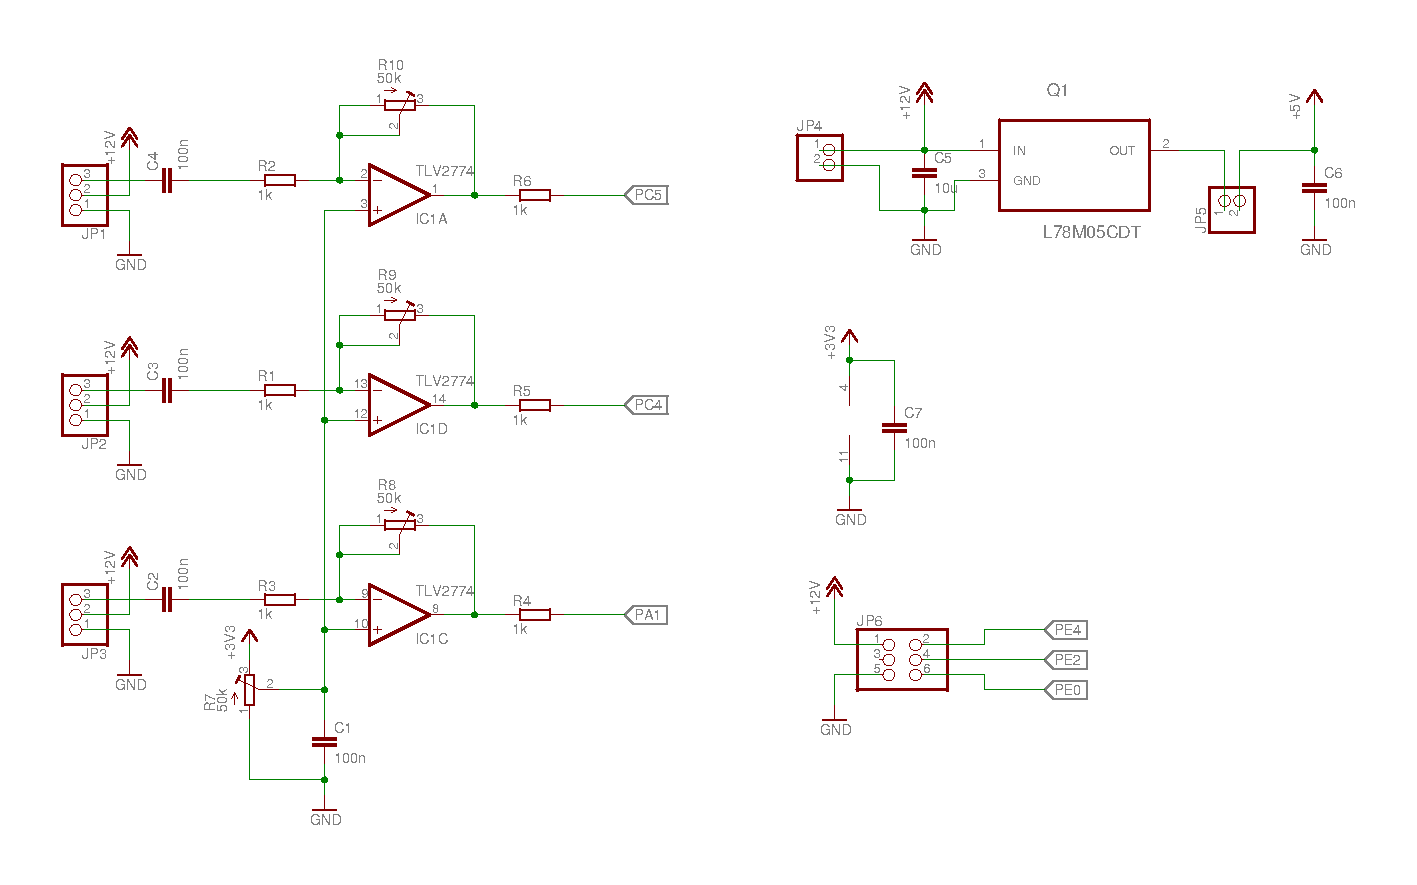
\includegraphics[width=1\textwidth, trim= 5mm 0mm 0mm 0mm,clip]{mainboard2}
    \caption{Schemat budowy przystawki do \textit{stm32f4-discovery}.}
    \label{fig:przystawka}
\end{figure}


